\subsubsection{テンプレートとは何か}
おそらくあなたはMVCのデザインパターンについて聞いたことがあると思います。Modelはデータを処理を、Viewは表示結果を、Controllerはユーザのリクエストの制御を行います。Viewレイヤーの処理では、多くの動的な言語ではどれも静的なHTMLの中に動的言語が生成したデータを挿入します。例えばJSPでは\texttt{<\%=....=\%>}を挿入することで、PHPでは\texttt{<?php.....?>}を挿入することで実現します。

下の図でテンプレートのメカニズムについてご紹介します

\begin{figure}[H]
  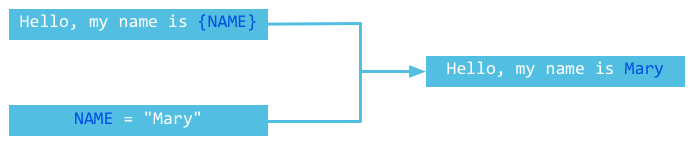
\includegraphics[width=14cm]{7.4.template.png}
   \label{図7.1}
   \caption{テンプレートのメカニズム図}
\end{figure}


Webアプリケーションがクライアントに返すフィードバックの情報の中の大部分の内容は静的で不変です。また少ない部分でユーザのリクエストによって動的に生成されるものがあります。例えばユーザのアクセスログリストを表示したい場合、ユーザ間ではログデータが異なるのみで、リストのスタイルは固定です。この時テンプレートを用いることで多くの静的なコードを使いまわすことができます。

\subsubsection{Goのテンプレートの使用}
Go言語では、\texttt{template}パッケージを使用してテンプレートの処理を行います。\texttt{Parse}、\texttt{ParseFile}、\texttt{Execute}といった方法を使ってファイルや文字列からテンプレートをロードします。その後植えの図で示したテンプレートのmerge操作のようなものを実行します。下の例をご覧ください:

\begin{lstlisting}[numbers=none]
func handler(w http.ResponseWriter, r *http.Request) {
    t := template.New("some template") //テンプレートを新規に作成する。
    t, _ = t.ParseFiles("tmpl/welcome.html", nil)  //テンプレートファイルを解析
    user := GetUser() //現在のユーザの情報を取得する。
    t.Execute(w, user)  //テンプレートのmerger操作を実行する。
}
\end{lstlisting}

上の例で、Go言語のテンプレート操作は非常に簡単で便利だとおわかりいただけるかと思います。その他の言語のテンプレート処理に似ていて、まずデータを取得した後データを適用します。

デモとテストコードの簡便のため、以降の例では以下の形式のコードを採用します。

\begin{itemize}
  \item ParseFilesの代わりにParseを使用します。Parseは直接文字列をテストでき、外部のファイルを必要としないためです。
  \item handlerを使ってデモコードを書くことはせず、それぞれひとつのmainをテストします。便利なテストです。
  \item \texttt{http.ResponseWriter}の代わりに\texttt{os.Stdout}を使用します。\texttt{os.Stdout}は\texttt{io.Writer}インターフェースを実装しているからです。
\end{itemize}


\subsubsection{どのようにしてテンプレートの中にデータを挿入するのか?}
上においてどのように解析とテンプレートの適用するかデモを行いました。以降ではさらに詳しくどのようにデータを適用していくのか理解していきましょう。テンプレートはすべてGoのオブジェクト上で適用されます。Goオブジェクトのフィールドはどのようにしてテンプレートの中に挿入されるのでしょうか?

\paragraph{フィールドの操作}
Go言語のテンプレートは\texttt{\{\{\}\}}を通して適用時に置換する必要のあるフィールドを含めます。\texttt{\{\{.\}\}}は現在のオブジェクトを示しています。これはJavaやC++の中のthisに似たものです。もし現在のオブジェクトのフィールドにアクセスしたい場合は\texttt{\{\{.FieldName\}\}}というようにします。ただし注意してください:このフィールドは必ずエクスポートされたものとなります(頭文字が大文字になります)、さもなければ適用時にエラーを発生させます。下の例をご覧ください:

\begin{lstlisting}[numbers=none]
package main

import (
    "html/template"
    "os"
)

type Person struct {
    UserName string
}

func main() {
    t := template.New("fieldname example")
    t, _ = t.Parse("hello {{.UserName}}!")
    p := Person{UserName: "Astaxie"}
    t.Execute(os.Stdout, p)
}
\end{lstlisting}

上のコードでは正しく\texttt{hello Astaxie}と出力されます。しかしもしコードに修正を加え、テンプレートにエクスポートされていないフィールドを含むと、エラーを発生させます。

\begin{lstlisting}[numbers=none]
type Person struct {
    UserName string
    email    string  //エクスポートされていないフィールド、頭文字が小文字です。
}

t, _ = t.Parse("hello {{.UserName}}! {{.email}}")
\end{lstlisting}

上のコードはエラーを発生させます。なぜならエクスポートされていないフィールドをコールしたためです。しかしもし存在しないフィールドをコールした場合はエラーを発生させず、空文字列を出力します。

テンプレートで\texttt{\{\{.\}\}}を出力すると、一般的には文字列オブジェクトに対して適用されます。デフォルトでfmtパッケージがコールされ文字列の内容が出力されます。



\paragraph{ネストしたフィールドの内容の出力}
上の例でどのようにひとつのオブジェクトのフィールドを出力するか示しました。もしフィールドの中にまたオブジェクトがある場合は、どのようにループしてこれらの内容を出力するのでしょうか?ここでは\texttt{\{\{with ...\}\}...\{\{end\}\}}と\texttt{\{\{range ...\}\}\{\{end\}\}}によってデータを出力することができます。

\begin{itemize}
  \item \{\{range\}\} はGo言語の中のrangeに似ています。ループしてデータを操作します
  \item \{\{with\}\}操作は現在のオブジェクトの値を指します。コンテキストの概念に似ています。
\end{itemize}

詳細な使用方法は以下の例をご覧ください:

\begin{lstlisting}[numbers=none]
package main

import (
    "html/template"
    "os"
)

type Friend struct {
    Fname string
}

type Person struct {
    UserName string
    Emails   []string
    Friends  []*Friend
}

func main() {
    f1 := Friend{Fname: "minux.ma"}
    f2 := Friend{Fname: "xushiwei"}
    t := template.New("fieldname example")
    t, _ = t.Parse(`hello {{.UserName}}!
            {{range .Emails}}
                an email {{.}}
            {{end}}
            {{with .Friends}}
            {{range .}}
                my friend name is {{.Fname}}
            {{end}}
            {{end}}
            `)
    p := Person{UserName: "Astaxie",
        Emails:  []string{"astaxie@beego.me", "astaxie@gmail.com"},
        Friends: []*Friend{&f1, &f2}}
    t.Execute(os.Stdout, p)
}
\end{lstlisting}

\paragraph{条件分岐}
Goテンプレートにおいてもし条件判断が必要となった場合は、Go言語の\texttt{if-else}文に似た方法を使用することで処理することができます。もしpipelineが空であれば、ifはデフォルトでfalseだと考えます。下の例でどのように\texttt{if-else}文を使用するか示します:


\begin{lstlisting}[numbers=none]
package main

import (
    "os"
    "text/template"
)

func main() {
    tEmpty := template.New("template test")
    tEmpty = template.Must(tEmpty.Parse(
        "空の pipeline if demo: {{if ``}} 出力されません。 {{end}}\n"))
    tEmpty.Execute(os.Stdout, nil)

    tWithValue := template.New("template test")
    tWithValue = template.Must(tWithValue.Parse(
        "空ではない pipeline if demo: {{if `anything`}} コンテンツがあります
        。出力します。 {{end}}\n"))
    tWithValue.Execute(os.Stdout, nil)

    tIfElse := template.New("template test")
    tIfElse = template.Must(tIfElse.Parse("if-else demo:
               {{if `anything`}} if部分 {{else}} else部分.{{end}}\n"))
    tIfElse.Execute(os.Stdout, nil)
}
\end{lstlisting}

上のデモコードを通して\texttt{if-else}文が相当簡単であることがわかりました。使用に際してとても簡単にテンプレートコードの中に集約されます。

\begin{quote}
注意:ifの中では条件判断を使用することができません。例えば、\texttt{Mail=="astaxie@gmail.com"}のような判断は誤りです。ifの中ではbool値のみ使用できます。
\end{quote}

\paragraph{pipelines}
Unixユーザは\texttt{pipe}についてよくご存知でしょう。\texttt{ls | grep "beego"}のような文法はよく使われるものですよね。カレントディレクトリ以下のファイルをフィルターし、"beego"を含むデータを表示します。前の出力を後の入力にするという意味があります。最後に必要なデータを表示します。Go言語のテンプレートの最大のアドバンテージはデータのpipeをサポートしていることです。Go言語の中でいかなる\texttt{\{\{\}\}}の中はすべてpipelinesデータです。例えば上で出力したemailにもしXSSインジェクションを引き起こす可能性があるとすると、どのように変換するのでしょうか?

\begin{lstlisting}[numbers=none]
{{. | html}}
\end{lstlisting}

emailが出力される場所では上のような方法で出力をすべてhtmlの実体に変換することができます。上のような方法は我々が普段書いているUnixの方法とまったく一緒ではないですか。とても簡単に操作することができます。他の関数をコールする場合も似たような方法となります。


\paragraph{テンプレート変数}
ときどき、テンプレートを使っていてローカル変数を定義したい場合があります。操作の中でローカル変数を宣言することができます。例えば\texttt{with``range``if}プロセスではローカル変数を宣言します。この変数のスコープは\texttt{\{\{end\}\}}の前です。Go言語で宣言されたローカル変数の形式は以下のとおりです:


\begin{lstlisting}[numbers=none]
$variable := pipeline
\end{lstlisting}

詳細な例は以下をご覧ください:

\begin{lstlisting}[numbers=none]
{{with $x := "output" | printf "%q"}}{{$x}}{{end}}
{{with $x := "output"}}{{printf "%q" $x}}{{end}}
{{with $x := "output"}}{{$x | printf "%q"}}{{end}}
\end{lstlisting}


\paragraph{テンプレート関数}
テンプレートがオブジェクトのフィールドの値を出力する際、\texttt{fmt}パッケージを採用してオブジェクトを文字列に変換します。しかしときどき我々はこうしたくはないときもあります。例えばスパムメールの送信者がウェブページから拾い集めてくる方法で我々のメールボックスへ情報を送信することを防止したいときがあります。\texttt{@}をatに変換したいわけです。たとえば:\texttt{astaxie at beego.me}のように。このような機能を実装したい場合は、自分で定義した関数でこの機能を作成する必要があります。

各テンプレート関数はいずれも単一の名前をもっていて、一つのGo関数と関係しています。以下の方法によって関係をもたせます。


\begin{lstlisting}[numbers=none]
type FuncMap map[string]interface{}
\end{lstlisting}

例えば、もしemail関数のテンプレート関数の名前を\texttt{emailDeal}としたい場合は、これが関係するGo関数の名前は\texttt{EmailDealWith}となります。下の方法でこの関数を登録することができます。

\begin{lstlisting}[numbers=none]
t = t.Funcs(template.FuncMap{"emailDeal": EmailDealWith})
\end{lstlisting}

\texttt{EmailDealWith}という関数の引数と戻り値は以下のように定義します:

\begin{lstlisting}[numbers=none]
func EmailDealWith(args ...interface{}) string
\end{lstlisting}

以下の実装例を見てみましょう:

\begin{lstlisting}[numbers=none]
package main

import (
    "fmt"
    "html/template"
    "os"
    "strings"
)

type Friend struct {
    Fname string
}

type Person struct {
    UserName string
    Emails   []string
    Friends  []*Friend
}

func EmailDealWith(args ...interface{}) string {
    ok := false
    var s string
    if len(args) == 1 {
        s, ok = args[0].(string)
    }
    if !ok {
        s = fmt.Sprint(args...)
    }
    // find the @ symbol
    substrs := strings.Split(s, "@")
    if len(substrs) != 2 {
        return s
    }
    // replace the @ by " at "
    return (substrs[0] + " at " + substrs[1])
}

func main() {
    f1 := Friend{Fname: "minux.ma"}
    f2 := Friend{Fname: "xushiwei"}
    t := template.New("fieldname example")
    t = t.Funcs(template.FuncMap{"emailDeal": EmailDealWith})
    t, _ = t.Parse(`hello {{.UserName}}!
                {{range .Emails}}
                    an emails {{.|emailDeal}}
                {{end}}
                {{with .Friends}}
                {{range .}}
                    my friend name is {{.Fname}}
                {{end}}
                {{end}}
                `)
    p := Person{UserName: "Astaxie",
        Emails:  []string{"astaxie@beego.me", "astaxie@gmail.com"},
        Friends: []*Friend{&f1, &f2}}
    t.Execute(os.Stdout, p)
}
\end{lstlisting}

上ではどのように自分で関数を定義するかお見せしました。実は、テンプレートパッケージの内部ではすでにビルトインの関数が実装されています。下のコードを切り取って自分のテンプレートパッケージの中にはりつけてください。

\begin{lstlisting}[numbers=none]
var builtins = FuncMap{
    "and":      and,
    "call":     call,
    "html":     HTMLEscaper,
    "index":    index,
    "js":       JSEscaper,
    "len":      length,
    "not":      not,
    "or":       or,
    "print":    fmt.Sprint,
    "printf":   fmt.Sprintf,
    "println":  fmt.Sprintln,
    "urlquery": URLQueryEscaper,
}
\end{lstlisting}


\subsubsection{Must操作}
テンプレートパッケージには\texttt{Must}という関数があります。この作用はテンプレートが正しいか検査することです。例えば大括弧が揃っているか、コメントは正しく閉じられているか、変数は正しく書かれているかといったことです。ここでは例を一つお見せします。Mustを使ってテンプレートが正しいか判断します:


\begin{lstlisting}[numbers=none]
package main

import (
    "fmt"
    "text/template"
)

func main() {
    tOk := template.New("first")
    template.Must(tOk.Parse(" some static text /* and a comment */"))
    fmt.Println("The first one parsed OK.")

    template.Must(template.New("second").
                           Parse("some static text {{ .Name }}"))
    fmt.Println("The second one parsed OK.")

    fmt.Println("The next one ought to fail.")
    tErr := template.New("check parse error with Must")
    template.Must(tErr.Parse(" some static text {{ .Name }"))
}
\end{lstlisting}

出力は以下の内容となります:

\begin{lstlisting}[numbers=none]
The first one parsed OK.
The second one parsed OK.
The next one ought to fail.
panic: template: check parse error with Must:1: unexpected "}" in command
\end{lstlisting}


\subsubsection{ネストしたテンプレート}
Webアプリケーションを作る時はテンプレートの一部が固定され不変である場合がよくあり、抜き出して独立した部分とすることができます。例えばブログのヘッダとフッタが固定で、変更があるのは真ん中のコンテンツの部分だけだとします。そのため\texttt{header}、\texttt{content}、\texttt{footer}の3つの部分として定義することができます。Go言語では以下のような文法によってこれを宣言します


\begin{lstlisting}[numbers=none]
{{define "サブテンプレートの名前"}}コンテンツ{{end}}
\end{lstlisting}

以下の方法によってコールします:

\begin{lstlisting}[numbers=none]
{{template "サブテンプレートの名前"}}
\end{lstlisting}

ここではどのようにしてネストしたテンプレートを使うかお見せします。3つのファイルを定義します。\texttt{header.tmpl}、\texttt{content.tmpl}、\texttt{footer.tmpl}ファイルです。内容は以下のとおり



\begin{lstlisting}[numbers=none]
//header.tmpl
{{define "header"}}
<html>
<head>
    <title>デモンストレーションの情報</title>
</head>
<body>
{{end}}

//content.tmpl
{{define "content"}}
{{template "header"}}
<h1>ネストのデモ</h1>
<ul>
    <li>ネストではdefineを使用してサブテンプレートを定義します。</li>
    <li>templateの使用をコール</li>
</ul>
{{template "footer"}}
{{end}}

//footer.tmpl
{{define "footer"}}
</body>
</html>
{{end}}
\end{lstlisting}

デモコードは以下の通り:

\begin{lstlisting}[numbers=none]
package main

import (
    "fmt"
    "os"
    "text/template"
)

func main() {
    s1, _ := template.ParseFiles("header.tmpl",
                                 "content.tmpl", "footer.tmpl")
    s1.ExecuteTemplate(os.Stdout, "header", nil)
    fmt.Println()
    s1.ExecuteTemplate(os.Stdout, "content", nil)
    fmt.Println()
    s1.ExecuteTemplate(os.Stdout, "footer", nil)
    fmt.Println()
    s1.Execute(os.Stdout, nil)
}
\end{lstlisting}

上の例で\texttt{template.ParseFiles}を使ってすべてのネストしたテンプレートをテンプレートの中にパースできることがお分かりいただけたかと思います。各定義の{{define}}はすべて独立した一個のテンプレートで、互いに独立しています。並列して存在している関係です。内部ではmapのような関係(keyがテンプレートの名前で、valueがテンプレートの内容です。)が保存されています。その後\texttt{ExecuteTemplate}を使って対応するサブテンプレートの内容を実行します。headerとfooterのどちらも互いに独立していることがわかります。どれもコンテンツを出力できます。contentの中でheaderとfooterのコンテンツがネストしているので、同時に3つの内容を出力できます。しかし、\texttt{s1.Execute}を実行した時、何も出力されません。デフォルトではデフォルトのサブテンプレートが無いからです。そのため何も出力されません。

\begin{quote}
単一の集合のようなテンプレートは互いを知っています。もしあるテンプレートが複数の集合によって使用された場合、複数の集合の中で別々にパースされる必要があります。
\end{quote}

\subsubsection{まとめ}
テンプレートに対する上記の詳細な紹介で、どのようにして動的なデータとテンプレートを融合させるかご理解いただけたかと思います:ループしたデータの出力、関数を定義、テンプレートのネスト等々。テンプレートの技術を応用することで、MVCパターンのVの処理を完成させることができます。以降の章ではどのようにMとCを処理するかご紹介します。

